\section{Élimination du mouvement libre}
\begin{frame}
  	\frtt{Recherche du mouvement libre}
  	\textbf{Objectif :} éliminer les contributions géophysiques du signal.
  	\vfil
	\textbf{Analyse :} addition de terme périodique avec amplitudes ajustées, décomposition de la nutation par FFT :

  	\centerline{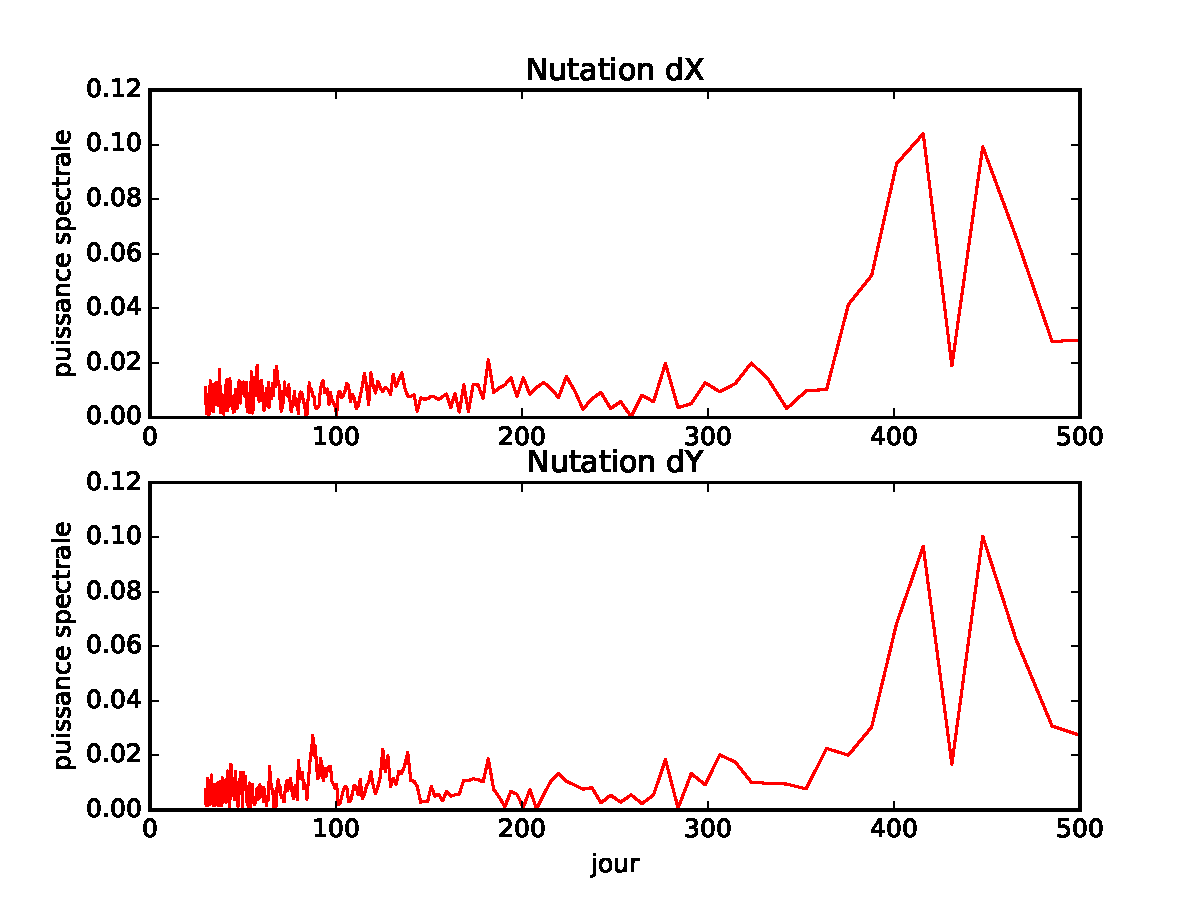
\includegraphics[scale=0.3]{original_frequence_nutation.pdf}}
  	\onslide<2->{$\implies$ apparition du terme libre à 457j}
\end{frame}

\begin{frame}
  \frtt{Nettoyage du terme libre}
  \begin{itemize}
      \onslide<1->
    \item Terme empirique : $ \tilde{A}_t \exp\left( \frac{2\pi }{457 \mbox{jours}}i \times t  \right) $
      \onslide<2->
    \item Ajustement du terme $ \tilde{A}_t $ sur une fenêtre centrée sur $t$ 
      \onslide<3->
    \item Déplacement de la fenêtre et interpolation : $ \tilde{A}_t\ \forall\ t $
  \end{itemize}

  \onslide<4->
  \centerline{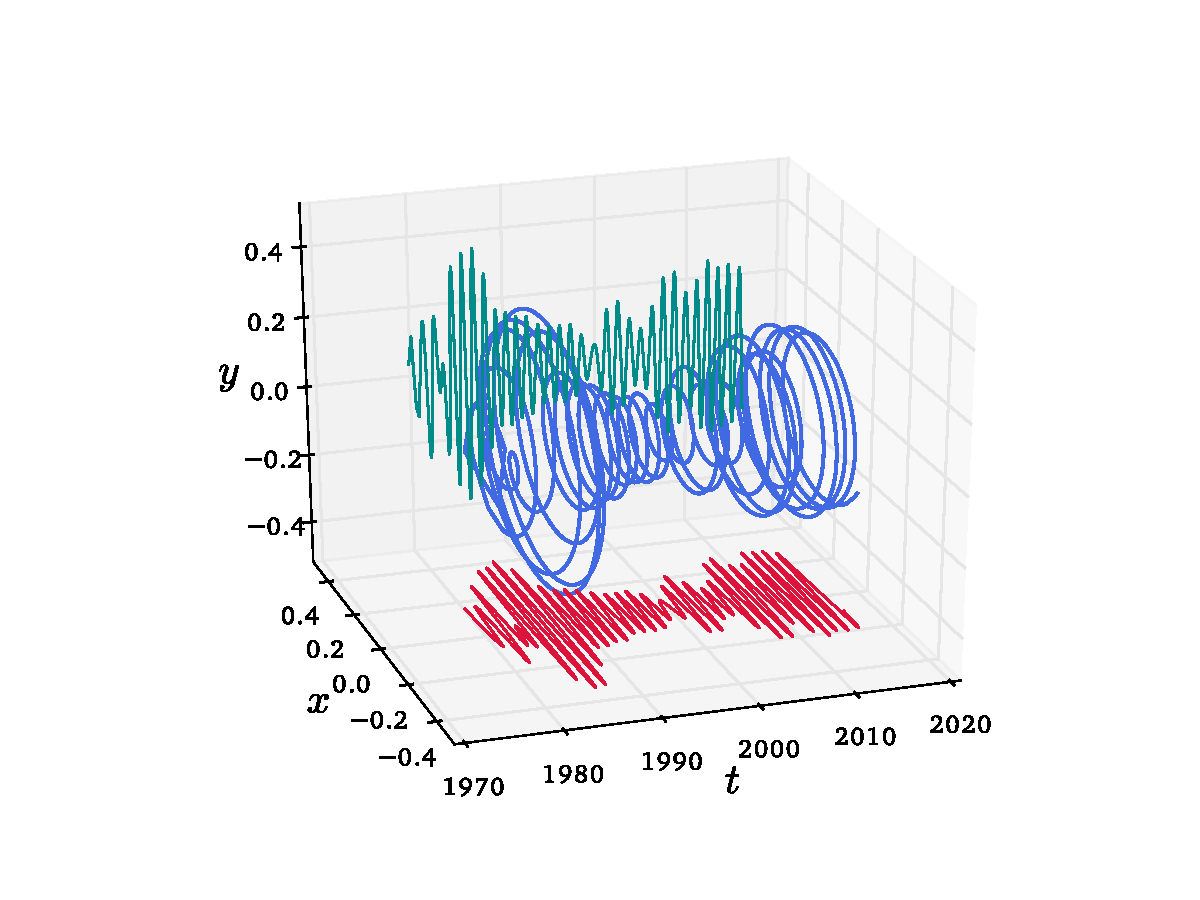
\includegraphics[scale=0.4]{free_wobble_manuel.pdf}}
\end{frame}


\begin{frame}
  \frtt{Signal Nettoyé}
  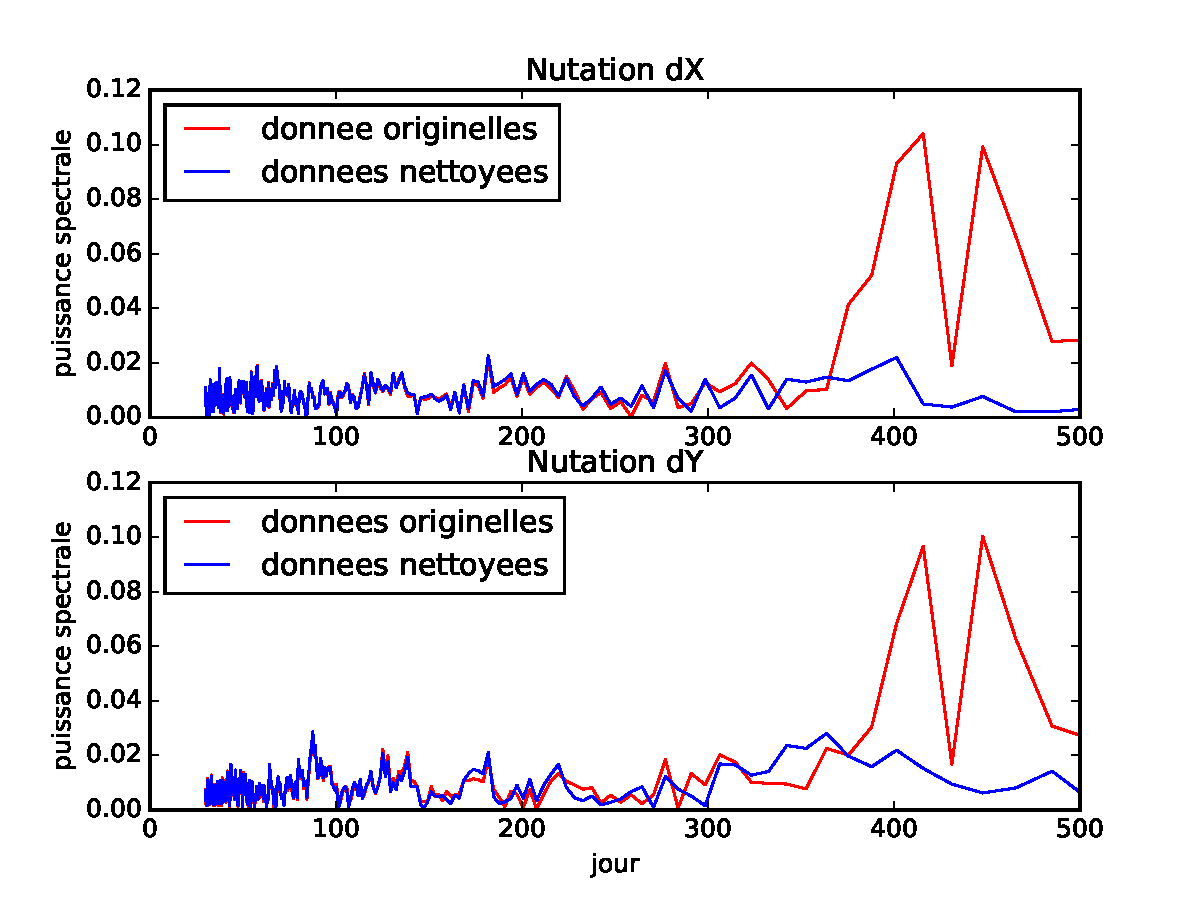
\includegraphics[scale=0.5]{frequence_nutation.pdf}
\end{frame}

